\newpage
\chapter{Verwendete Daten}

\section{Numenta Zeitreihen Daten}
\label{sec:numTS}
Bei diesem Datensatz handelt es sich um k�nstlich erzeugte Zeitreihen der Numenta Gruppe. Diese Zeitreihen enthalten unterschiedliche Arten von Ausrei�ern. Dadurch kann untersucht werden f�r welche Ausrei�er Typen die Algorithmen gut geeignet sind. F�r die Tests auf multivariaten Zeitreihen wurden neue Zeitreihen erzeugt. Dabei wurde f�r die erste Dimension eine Zeitreihe der Numenta Gruppe verwendet. F�r weitere Dimensionen wurde auf eine Zeitreihe ohne Ausrei�er zur�ck gegriffen \cite{AHMAD2017134}.

\begin{figure}[H]
	\centering
	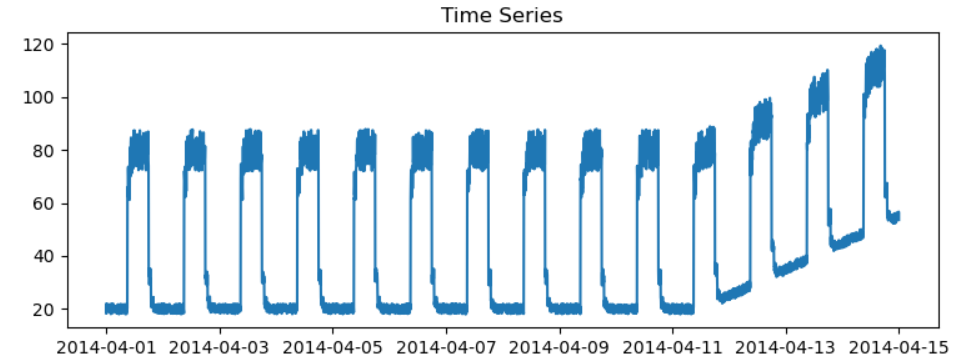
\includegraphics[width=10cm]{fig/numentaExample.PNG}
	\caption{Beispielzeitreihe Numenta}
	\label{img:numentaTS}
\end{figure}


\section{Netzwerk-Datens�tze}

Im Forschungsgebiet der Ausrei�er-Erkennung in Graphen herrscht eine starke Konkurrenz unter den wenigen Forschern. Aus diesem Grund finden sich zum Gro�teil der ver�ffentlichten Paper, sowie Code, keine gelabelten Datens�tze. Diese werden, um den eigenen Vorteil nicht zu verlieren, zur�ckgehalten f�r die eigene Forschung. \workTodo{Paper finden und Quelle einf�gen zu dieser Problematik}

Im Rahmen des Forschungsprojekts konnten zwei Datens�tze verwendet werden deren Ausrei�er in unterschiedlichen Formen deklariert wurden. Diese Datens�tze werden im Folgenden vorgestellt.
 
\subsubsection{Enron}

Der Enron Datensatz enth�lt die intern versendeten E-Mail Daten von rund 150 Mitarbeitern der Firma Enron. Die Daten wurden von der Federal Energy Regulatory Commission offengelegt. Enthalten sind ca. 50.000 E-Mail-Nachrichten. F�r den Algorithmus wird lediglich der Zeitpunkt, an dem eine E-Mail versendet wird, sowie die Sender und Empf�nger festgehalten.

Die Messung der Ausrei�er erfolgt in zwei Schritten. Zum einen werden Erkenntnisse aus dem Schaubild des SEDANSPOT-Algorithmus gewonnen \workTodo{Quelle eingeben}. 
Im n�chsten Schritt wird die selbe Vorgehensweise wie aus dem SEDANSPOT-Paper gew�hlt und die ENRON Timeline \workTodo{Quelle einf�gen} zur Erhebung von m�glichen Auswirkungen f�r die Ausrei�er hinzugezogen.


\subsubsection{DARPA}

Der DARPA-Datensatz \citep{DARPA} beinhaltet 4.5 Millionen IP zu IP Kommunikationen zwischen 9.4 Tausend Quell-IP's und 23.3 Tausend Ziel-IP's �ber einen Zeitraum von 87.7 Tausend Minuten. Jede Kommunikation ist eine gerichtete Kante von der Quell-IP zur Ziel-IP in einem Zeitpunkt. Eine vierte Spalte des Datensatzes ist verf�gbar, in der ein \textit{label} enthalten bzw. ein Angriff gekennzeichnet ist. Der DARPA-Datensatz besteht zu �ber 60\% aus Ausrei�ern. 
\workTodo{Quelle zum Datensatz einf�gen} 
